\documentclass{standalone}
\usepackage{mathpazo}
\usepackage[american voltages]{circuitikz}

\begin{document}
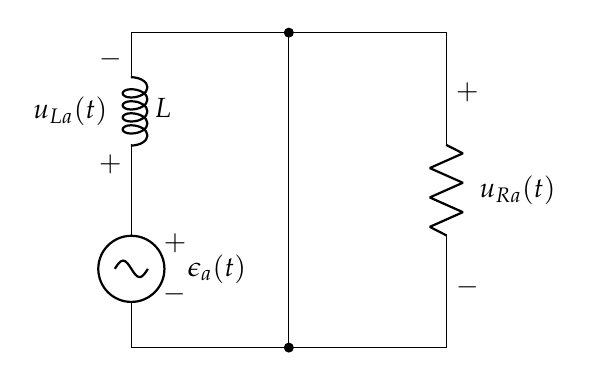
\begin{tikzpicture}
  \coordinate (A) at (0,4);
  \coordinate (B) at (2,4);
  \coordinate (C) at (4,4);
  \coordinate (D) at (0,0);
  \coordinate (E) at (2,0);
  \coordinate (F) at (4,0);
  \draw
  (A) to [short] (B)
  to [short] (C)
  to [R, v^=$u_{Ra}(t)$] (F);
  \draw
  (F) to [short] (E)
  to [short] (D);
  \draw
  (A)   to [L, l=$L$, v<=$u_{La}(t)$] ++(0,-2)
  to [sV, v=$\epsilon_a(t)$] (D);
  \draw
  (B) to [short, *-*] (E);
  \end{tikzpicture}
\end{document}